\section{Response to interannual ENSO variability}

This section describes the synchronous response of the epipelagic community simulated by the model to ENSO variability in the tropical Pacific. We first discuss the response to the iconic 1997/1998 El Niño and then generalise these results to the overall ENSO variability. 

\subsection{The iconic 1997/1998 El Niño event}

We first focus on the 1997/98 El Niño event because (1) it is the strongest El Niño event on records (Santoso et al. 2017) and (2) the ocean response to this specific event has been extensively described and analyzed, in terms of physics  (e.g. \cite{mcphadenGenesisEvolution1997981999, vialardModelStudyOceanic2001, lengaigneOceanResponseMarch2002}, biogeochemistry \citep{chavezBiologicalChemicalResponse1999a, gierachBiologicalResponse19972012} and ecosystems (e.g. \cite{leaObservationsFishesAssociated2000, glynnCoralBleachingMortality2001,arcosJackMackerelFishery2001}).

Figure \ref{fig:mean_ond97_ape} displays the mean biomass density over the 1958-2018 period (left column) and the biomass density anomalies averaged over the 97 October, November and December (OND) months, when the El Nino signal is at its maximum.

\begin{figure}
	\centering
	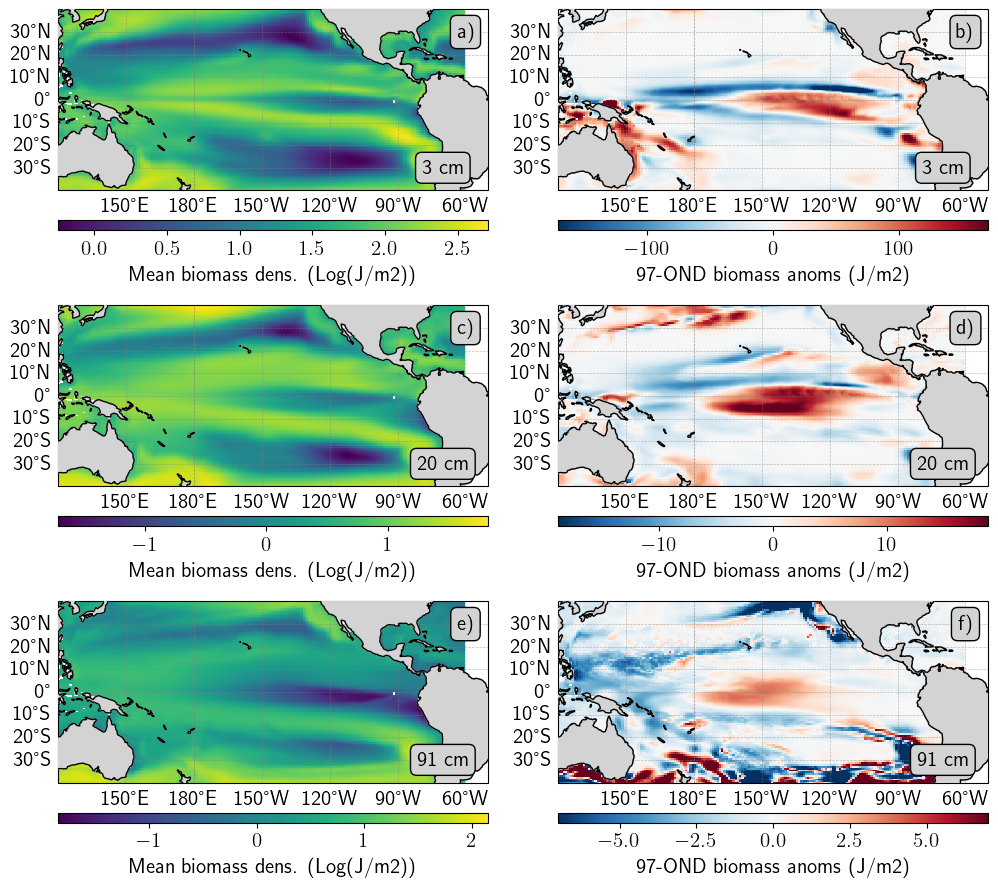
\includegraphics[scale=0.5]{figs/fig3.png}	
	\caption{Mean fish biomass (left column, log-scale) and OND-97 anomalies for small (upper line), intermediate (middle line) and large sizes (lower line).}	
	\label{fig:mean_ond97_ape}
\end{figure}

For small sizes (Figure \ref{fig:mean_ond97_ape}a), the mean fish biomass is concentrated at around 10° S and 10°N in the central Pacific and close to the equator in the western Pacific. High biomass concentration is also found east of 90° W, off the coasts of Chile. As size increases, the equatorial "blue spot" extends meridionally and to the west. This pattern is mostly driven by the active and passive advection of fishes in the Apecosm model. Without advection, the biomass will be concentrated at the equator, where the plankton concentration is the maximum.

During the 97 El Nino, small epipelagics show negative anomalies in the Western Equatorial Pacific and positive anomalies in the Central Equatorial Pacific. This pattern can be interpreted as an eastern displacement of the mean biomass in the Western Pacific. Similar dipolar patterns are also obtained for intermediate and large sizes, but the anomalies shift westward as size increases. This can be interpreted, as for small sizes, by a westward shift of fish biomass during positive El Niño phases.

\warn{Discussion of the profiles???}

\begin{figure}
	\centering
	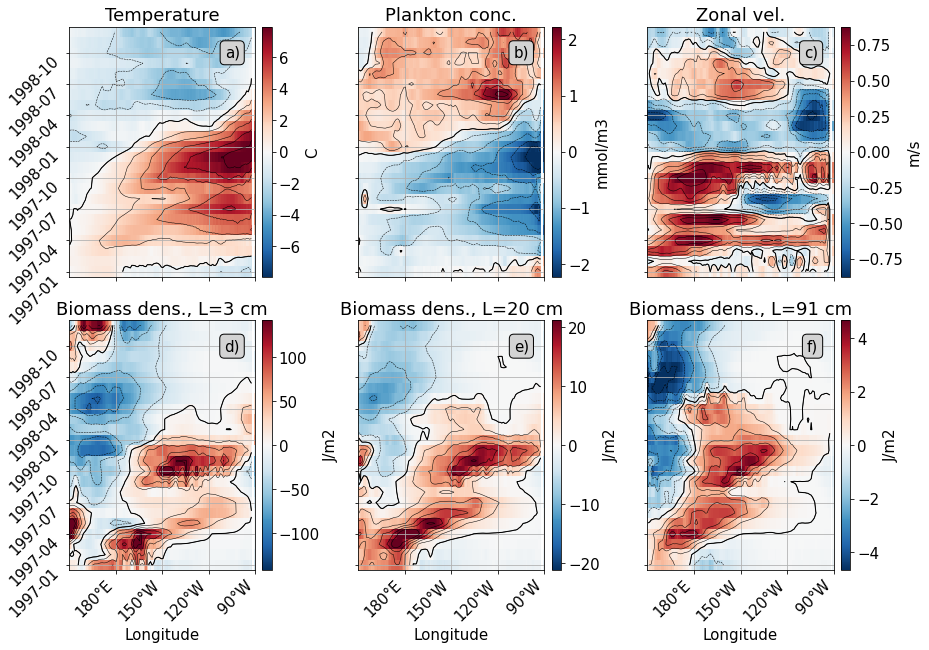
\includegraphics[scale=0.4]{figs/fig5.png}	
	\caption{Hovmoller diagrams of equatorial temperature (a), low-trophic level concentrations (b), zonal velocity (c) and fish biomass anomalies (3cm, 20cm and 90 cm in d, e, f, respectively).}	
	\label{fig:hov_nemo_ape}
\end{figure}

Figures \ref{fig:hov_nemo_ape}a, \ref{fig:hov_nemo_ape}b, \ref{fig:hov_nemo_ape}c display equatorial hovmüller diagrams of the temperature, chlorophyll and zonal currents anomalies averaged over the top 50m simulated by the ocean model during the 1997/1999 period. In agreement with observations (not shown; see \cite{lengaigneOceanResponseMarch2002}), the warming signal associated with the 1997 El Niño initiates in early spring over the central and eastern equatorial Pacific, peaks by the end of the calendar year in the eastern Pacific to quickly recede and switches La Niña conditions the following spring (Figure \ref{fig:hov_nemo_ape}a). The El Niño warming period is accompanied by strong surface eastward anomalous currents (Figure \ref{fig:hov_nemo_ape}c) promoted by anomalous westerly winds and contributing to central Pacific warming and eastward shift of the warm-pool towards the eastern equatorial Pacific. These current anomalies reverse during La Niña. Simulated plankton concentration anomalies tend to mirror temperature anomalies, with a strong decline during El Niño and an enhanced bloom during La Niña (Figure \ref{fig:hov_nemo_ape}.b). 

The same analysis is then performed for epipelagic biomass for the three targeted size classes (Fig\ref{fig:hov_nemo_ape}d, Fig\ref{fig:hov_nemo_ape}e and Fig\ref{fig:hov_nemo_ape}f), which share some common features: positive biomass anomalies for the three communities appear near the dateline in early spring and propagate eastward towards the central Pacific until the end of summer. Another positive patch then develops in the central Pacific in fall and quickly recedes in winter. These positive anomalies in the central and eastern Pacific  are associated with negative biomass anomalies in the western Pacific during the 1997/98 El Niño. These negative anomalies persist after the El Niño demise and during the following La Niña event but remain restricted to the western Pacific. While sharing similarities, the response of larger epipelagic fishes is generally shifted westward compared to smaller ones.



